\documentclass{book}
\usepackage{xeCJK}
\usepackage{ctexcap}
\usepackage{bm}
\usepackage{amsmath,amssymb,amsfonts}
\usepackage{float}

\begin{document}
\chapter{变压器的运行原理和主要特性}
本章主要讨论变压器的运行原理、分析方法、参数及运行性能。首先分析变压器空载和负载运行时的电磁过程,导出变压器的基本方程式。再通过归算,导出变压器的等效电路和相量图,最后分析变压器的运行性能——电压变化率和效率。

研究过程中,为了突出主要因素,常常忽略某些次要因素的影响,在获得基本规律之后,再把忽略掉的次要因素考虑进去,以形成一个完整的概念。

本章以单相变压器为例讨论上述问题,但所得结论完全适用于三相变压器在对称负载下运行时每一相的情况。因此,这一章是变压器全篇的核心内容。

\section{变压器的空载运行}
空载是指变压器的一次侧接于电源,二次侧不接负载。
\subsection{电磁物理现象}
图\ref{fig:3.1}所示为一台单相变压器空载运行时的示意图。一、二次侧的匝数分别为${{N}_{1}}$和${{N}_{2}}$。把一次侧接到电压为${{u}_{1}}$的交流电网上时,一次侧中便有电流${{i}_{1}}$流过,这个电流称为变压器的空载电流,用${{i}_{0}}$表示,即${{i}_{1}}={{i}_{0}}$。空载电流完全用以励磁,故空载电流即励磁电流,用${{i}_{m}}$表示,即${{i}_{0}}={{i}_{m}}$。励磁电流产生交变磁动势${{i}_{m}}{{N}_{1}}$建立交变磁场。这个磁场的分布情况实际上是很复杂的。为了便于研究问题,把磁通分为两部分,如\ref{fig:3.1}所示。其中一部份磁通$\phi$沿铁心闭合,同时与一、二次侧相交链,是变压器进行能量传递的媒介,称为主磁通或互感磁通;另一部分通${{\phi }_{1\sigma }}$主要沿非铁磁材料闭合(沿变压器油或空气闭合)),仅与一次侧相交链,称为一次侧的漏磁通。由于铁心是由高导磁材料硅钢片制成的,导磁系数远比空气大,所以空载运行时,主磁通占总磁通的绝大部分,而漏磁通只占很小部分,约 0.1\%\textasciitilde0.2\%。可见,主磁通和漏磁通的作用和性质都不相同,主要表现在:由于铁磁材料存在饱和现象,主磁通与建立它的电流之间的关系是非线性的,即$\phi$与${{i}_{0}}$不是正比关系;但漏磁通由于主要沿非铁磁材料闭合,它与电流${{i}_{0}}$保持线性关系。另外,主磁通在一、二次侧内感应电动势,二次侧如果与负载接通,则在电动势的作用下向负载输出电功率,所以主磁通起传递能量的媒介作用;而漏磁通仅在一次侧内感应电动势,只起感抗压降的作用,不能传递能量。在分析变压器时,把这两种磁通分开,即可把非线性和线性问题分别处理,又便于分析它们所起的不同作用。

此外,空载电流还在一次侧中产生电阻压降。综上所述,把空载运行时所发生的电磁现 象汇总如图\ref{fig:3.2}所示,其中虚框内为磁量,虚框外为电量。
\begin{figure}  %两个图片并排放
	\begin{minipage}[H]{0.45\linewidth}  
		\centering  
		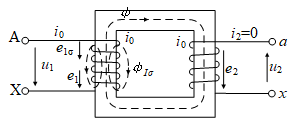
\includegraphics[width=2in]{3-1g.png}  
		\caption{单相变压器空载运行的示意图}
		\label{fig:3.1} 
	\end{minipage}
	\begin{minipage}[H]{0.45\linewidth}  
		\centering  
		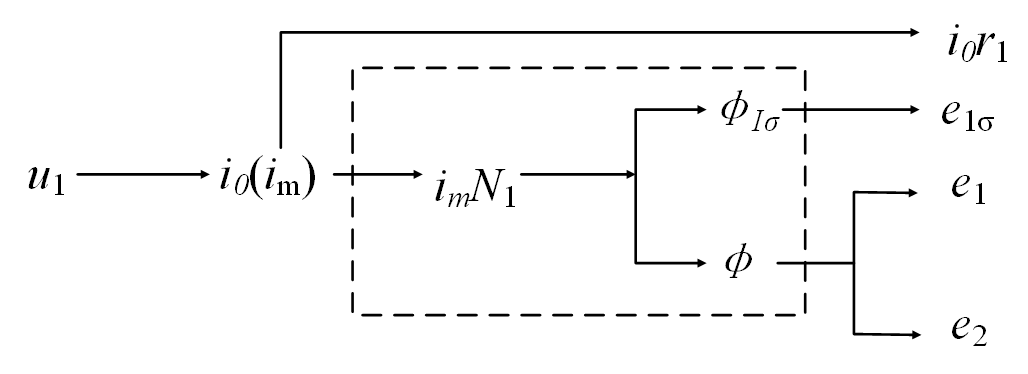
\includegraphics[width=2in]{3-2gai.png}  
		\caption{变压器空载运行时的电磁关系} 
		\label{fig:3.2} 
	\end{minipage}
\end{figure} 
\subsection{基本方程式}
\subsubsection{正方向的规定}
因为变压器的电压、电流、电动势、磁动势和磁通都是时间函数,是正负交替变化的物理量,在列方程式时,需先给它们规定正方向。否则所列出的方程,其物理意义便含混不清。所以在电路图中,都需要用箭头标出各物理量的正方向。

从理论上讲,正方向可以任意规定。选择不同的正方向,则所列出的表达式各异,但各 物理量的真实变化规律并不依正方向的选择不同而改变。

在电机理论中,通常按电工惯例规定正方向。这样,不仅便于文献交流,也可避免出现 误解。习惯上规定电流的正方向与该电流所产生磁通正方向应符合右手螺旋定则;规定磁通 的正方向与其感应电动势的正方向应符合右手螺旋定则。在图\ref{fig:3.1}中,各物理量的正方向就是按这个原则规定的。
\subsubsection{电压平衡方程式}
根据电磁感应定律,当磁通$\phi$和${{\phi }_{1\sigma }}$交变时,就分别在它们所交链的线圈内感应出电动 势,即
\[{{e}_{1}}=-{{N}_{1}}\frac{\text{d}\phi }{\text{d}t}\]
\[{{e}_{2}}=-{{N}_{2}}\frac{\text{d}\phi }{\text{d}t}\]
\[{{e}_{1\sigma }}=-{{N}_{1\sigma }}\frac{\text{d}{{\phi }_{1\sigma }}}{\text{d}t}\]
式中   ${{e}_{1}}$——主磁通$\phi$在一次侧感应的自感电动势的瞬时值;

${{e}_{2}}$——主磁通$\phi$在二次侧感应的互感电动势的瞬时值;

${{e}_{1\sigma }}$——漏磁通在一次侧感应的漏感电动势的瞬时值。

根据基尔霍夫第二定律,一次侧的电压方程式为
\begin{equation}
{{u}_{1}}=-\left( {{e}_{1}}+{{e}_{1\sigma }} \right)+{{i}_{0}}{{r}_{1}}
\label{2-1}
\end{equation}
当上述各物理量均按正弦规律变化时,则可写成复数形式,即
\begin{equation}
{{\dot{U}}_{1}}=-\left( {{{\dot{E}}}_{1}}+{{{\dot{E}}}_{1\sigma }} \right)+{{\dot{I}}_{0}}{{r}_{1}}
\label{2-2}
\end{equation}
二次侧电压方程式为
\begin{equation}
{{u}_{20}}={{e}_{2}}
\label{2-3}
\end{equation}
同样,其复数形式为
\begin{equation}
{{{\dot{U}}_{20}}={{\dot{E}}_{2}}}
\label{2-4}
\end{equation}

\subsection{电动势与变比}
首先研究主磁通所感应的电动势${{e}_{1}}$。由于漏磁通远小于主磁通,故${{e}_{1\sigma }}\ll {{e}_{1}}$。通常一次侧空载电流的电阻压降也很小,即${{i}_{0}}{{r}_{1}}\ll {{e}_{1}}$。因此,一次侧电压平衡方程式可近似地简化为${{u}_{1}}=-{{e}_{1}}$ 。如外施电压${{u}_{1}}$按正弦规律变化,则$\phi $、${{e}_{1}}$、${{e}_{2}}$也都按正弦规律变化。设
\[\phi ={{\Phi }_{m}}\sin \omega t\]
式中${{\Phi }_{m}}$——主磁通最大值;$\omega $——磁通的角频率,$\omega =2\pi f$

则
\begin{equation}
{{e}_{1}}=-{{N}_{1}}\frac{\text{d}\phi }{\text{d}t}=-\omega {{N}_{1}}{{\Phi }_{m}}\cos \omega t={{E}_{1m}}\sin \left( \omega t-90{}^\circ  \right)
\label{2-5}
\end{equation}
一次侧感应电动势的最大值为

\[{{E}_{1m}}=\omega {{N}_{1}}{{\Phi }_{m}}=2\pi f{{N}_{1}}{{\Phi }_{m}}\]
有效值为
\begin{equation}
{{E}_{1}}=\frac{{{E}_{1m}}}{\sqrt[{}]{2}}=4.44f{{N}_{1}}{{\Phi }_{m}}
\label{2-6}
\end{equation}
其复数形式为
\begin{equation}
{{\dot{E}}_{1}}=-\text{j}4.44f{{N}_{1}}{{\dot{\Phi }}_{m}}
\label{2-7}
\end{equation}
式\eqref{2-7}是计算变压器感应电动势的一个重要公式,它表示,感应电动势的大小与频率$f$、绕组匝数${{N}_{1}}$以及铁心中磁通的幅值${{\Phi }_{m}}$成正比例。当变压器接到额定频率的电网上运行时,由于$f$和${{N}_{1}}$均为常值,故电动势${{E}_{1}}$的大小仅由磁通${{\Phi }_{m}}$所决定。如前所述,当空载运行时,可以近似地认为外施电压${{u}_{1}}$仅由电动势${{e}_{1}}$ 所平衡,即在大小上${{U}_{1}}\approx {{E}_{1}}$,因此,这时主磁通${{\Phi }_{m}}$的大小可以近似地认为仅由外施电压${{U}_{1}}$的大小来确定,而与变压器所用的材料和尺寸无关。在图\ref{fig_3.3}(a)中,绘出了磁通及电动势随时间的变化波形。图\ref{fig_3.3}(a)中曲线清楚地显示出感应电动势落后于磁通90°,它们之间的相量关系如图\ref{fig_3.3}(b)所示。
\begin{figure}[H]
	\centering
	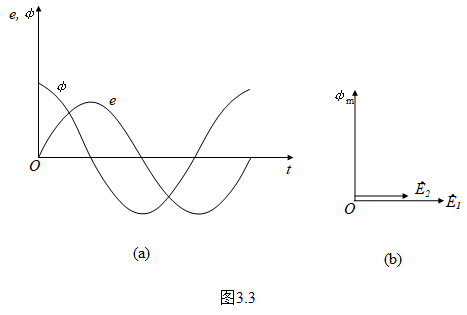
\includegraphics[width=0.80\textwidth]{3-3g.png}
	\caption{磁通及感应电势(a)波形图;(b)相量图}
	\label{fig_3.3}
\end{figure}
同样,也可得到二次侧的感应电动势为
\begin{equation}
{{E}_{2}}=4.44f{{N}_{2}}{{\Phi }_{m}}
\label{2-8}
\end{equation}
写成复数形式为
\begin{equation}
{{\dot{E}}_{2}}=-\text{j}4.44f{{N}_{2}}{{\dot{\Phi }}_{m}}
\label{2-9}
\end{equation}
因此,一次侧及二次侧的感应电动势之比为
\begin{equation}
\frac{{{E}_{1}}}{{{E}_{2}}}=\frac{{{N}_{1}}}{{{N}_{2}}}=k
\label{2-10}
\end{equation}
$k$就称为变压器的变比,它等于一、二次绕组的匝数比。当变压器空载运行时,由于一次侧${{U}_{1}}\approx {{E}_{1}}$,二次侧空载电压${{U}_{10}}\approx {{E}_{2}}$,故可近似地用一、二次侧电压之比作为变压器的变比,即
\begin{equation}
k=\frac{{{E}_{1}}}{{{E}_{2}}}\approx \frac{{{U}_{1}}}{{{U}_{20}}}
\label{2-11}
\end{equation}
从式\eqref{2-10}可以看出,只要只当地选择一、二次侧的匝数比,就可把电源供给的一次侧电压,变为所需的二次侧电压,这就是变压器的变压原理。

其次研究漏磁通的感应电动势。一次侧的漏磁链为
\[{{\psi }_{1\sigma }}\text{=}{{N}_{1}}{{\phi }_{1\sigma }}={{L}_{1\sigma }}{{i}_{0}}\]
式中${{L}_{1\sigma }}$——一次侧的漏磁电感,简称一次侧漏感。

由于漏磁通不饱和,可以认为${{\phi }_{1\sigma }}$和${{i}_{0}}$成正比,所以漏感${{L}_{1\sigma }}$是一个常数。漏磁通的感应电动势为
\[{{e}_{1\sigma }}=-{{N}_{1}}\frac{\text{d}{{\phi }_{1\sigma }}}{\text{d}t}=-{{L}_{1\sigma }}\frac{\text{d}{{i}_{0}}}{\text{d}t}\]
写成复数形式为
\begin{equation}
{{\dot{E}}_{1\sigma }}=-j\omega {{L}_{1\sigma }}{{\dot{I}}_{0}}=-j{{x}_{1\sigma }}{{\dot{I}}_{0}}
\label{2-12}
\end{equation}
式中  ${{x }_{1\sigma }}$——一次侧漏磁电抗,简称一次侧漏抗,${{x}_{1\sigma }}=\omega {{L}_{1\sigma }}$。
将式(\ref{2-10})带入式(\ref{2-2}),得到一次侧电压方程式为
\begin{equation}
{{\dot{U}}_{1}}=\left( -{{{\dot{E}}}_{1}} \right)+j{{\dot{I}}_{0}}{{x}_{1\sigma }}+{{\dot{I}}_{0}}{{r}_{1}}=\left( -{{{\dot{E}}}_{1}} \right)+{{\dot{I}}_{0}}{{Z}_{1}}
\label{2-13}
\end{equation}
式中  ${{Z}_{1}}$——一次侧的漏阻抗,${{Z}_{1}}={{r}_{1}}+j{{x}_{1\sigma }}$。空载时,一次侧阻抗压降${{\dot{I}}_{0}}{{Z}_{1}}$很小,因此外施电压${{U}_{1}}$的绝大部分与感应电动势$\left( -{{{\dot{E}}}_{1}} \right)$相平衡,即${{\dot{U}}_{1}}\approx \left( -{{{\dot{E}}}_{1}} \right)$。
\subsection{励磁电流的性质和波形}
在变压器空载运行时,一次侧的空载电流全部用来建主磁通,所以空载电流${{i}_{0}}$就是励磁电流${{i}_{m}}$。当外施正弦交流电压${{\dot{U}}_{1}}$时,为了产生与${{\dot{U}}_{1}}$相平衡的正弦电动势$\left( -{{{\dot{E}}}_{1}} \right)$,铁心中的主磁通必定也须按正弦规律交变。现在要讨论的是为建立这一正弦主磁通,电源需向变压器一次侧提供多大的励磁电流,励磁电流包含哪些成分。这将取决于变压器的铁心材料和几何尺寸.因为变压器的铁心材料是铁磁物质,故励磁电流的大小和波形将受到磁路饱和、磁滞和涡流的影响。下面对上述影响分别进行讨论。
\subsubsection{磁饱和对励磁电流的影响}
磁路的饱和程度取决于铁心中的磁通密度${{B}_{m}}$。

(1)若${{B}_{m}}<0.8T$,通常磁路处于未饱和状态,磁化曲线$\phi =f\left( {{i}_{0}} \right)$呈线性关系。当$\phi $按正弦规律变化时,产生它的${{i}_{0}}$也按正弦变化,相应波形可用作图法求出,如图\ref{fig_3.4}所示。因为未考虑铁损耗电流,励磁电流仅含磁化电流分量${{i}_{\mu }}$。
\begin{figure}[H]
	\centering
	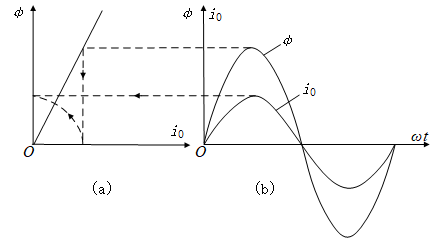
\includegraphics[width=0.80\textwidth]{3-4g.png}
	\caption{作图法求激磁电流(磁路不饱和)
		(a)磁化曲线;(b)磁通波和激磁电流波形}
	\label{fig_3.4}
\end{figure}
(2)若${{B}_{m}}>0.8T$,磁路开始饱和。$\phi  = f\left( {{i_0}}\right)$呈非线性,随导磁率逐渐变小。仍用作图法求励磁电流。当磁通$\phi$为正弦波时,${{i}_{0}}$ 为尖顶波,如图\ref{fig_3.5}所示。

尖顶的大小取决于饱和程度,磁路越饱和,尖顶的幅度越大。设计时常取${{B}_{m}}=\left( 1.4\tilde{\ }1.6 \right)T$,以免磁化电流幅值过大。同样,因为未考虑铁心损耗,励磁电流仅含磁化电流分量${{i}_{\mu }}$。

对尖顶波进行波形分解,除基波分量外,还包含各奇次谐波。其中以三次谐波幅值最大。在电路理论中,尖顶波电流不能用相量表示。为此,可用等效正弦波电流替代实际尖顶波磁化电流。等效原则是令等效正弦波与尖顶波有相同的有效值,与尖顶波的基波分项有相同频率且同相位。这样,磁化电流便可用相量${{\dot{I}}_{\mu }}$ 表示,${{\dot{I}}_{\mu }}$与${{\dot{\Phi }}_{m}}$ 同相位。因为${{\dot{E}}_{1}}$ 滞后于${{\dot{\Phi }}_{m}}$${{90}^{\text{o}}}$ ,故${{\dot{I}}_{\mu }}$滞后于$\left( -{{{\dot{E}}}_{1}} \right){{90}^{\text{o}}}$,${{\dot{I}}_{\mu }}$具有无功电流性质。它是励磁电流的主要成分。
\begin{figure}[H]
	\centering
	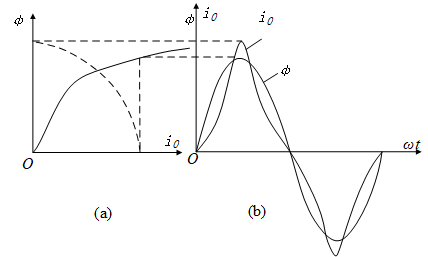
\includegraphics[width=0.80\textwidth]{3-5g.png}
	\caption{作图法求励磁电流(磁路饱和)(a)磁化曲线;(b)磁通波和励磁电流波形}
	\label{fig_3.5}
\end{figure}

\subsubsection{铁损耗对励磁电流的影响}
由于主磁通的交变,在铁心中将产生磁滞损耗和涡流损耗。电源除向变压器供给无功磁化电流${{\dot{I}}_{\mu }}$外,还要供给一定的有功电流。后者称为铁损耗电流,用${{\dot{I}}_{Fe}}$表示,它与$\left( -{{{\dot{E}}}_{1}} \right)$同相位,超前于主磁通${{\dot{\Phi }}_{m}}$${{90}^{\text{o}}}$,如图\ref{fig:3.6}所示。在变压器电路分析中,通常把励磁电流表示为磁化电流和铁损耗电流两个分量,即
\begin{equation}
{{\dot{I}}_{m}}={{\dot{I}}_{Fe}}+{{\dot{I}}_{\mu }}
\label{2-14}
\end{equation}

\begin{figure}  %两个图片并排放
	\begin{minipage}[H]{0.45\linewidth}  
		\centering  
		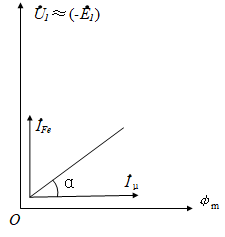
\includegraphics[width=2.2in]{3-6g.png}  
		\caption{励磁电流的两个分量}
		\label{fig:3.6} 
	\end{minipage}
	\begin{minipage}[H]{0.45\linewidth}  
		\centering  
		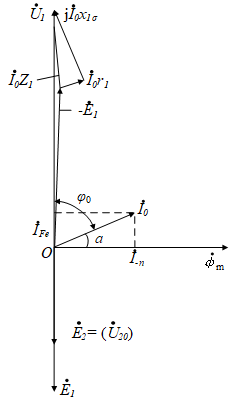
\includegraphics[width=2.2in]{3-7g.png}  
		\caption{变压器空载相量图} 
		\label{fig:3.7} 
	\end{minipage}
\end{figure}
变压器空载运行时,虽然二次侧没有功率输出,但一次侧仍要从电网吸取一部分有功功率来补偿由于磁通交变在铁心内引起的铁损耗和由于在一次侧内流过而引起的铜损耗。对电力变压器来说,空载损耗不超过额定容量的1\%,空载电流约为额定电流的2\% \textasciitilde10\%,上述值均随变压器量的增大而下降。

\subsection{相量图}
通过以上分析可得出变压器空载运行时的基本关系式为
\begin{equation}
\left. \begin{aligned}
& {{{\dot{I}}}_{0}}={{{\dot{I}}}_{m}}={{{\dot{I}}}_{Fe}}+{{{\dot{I}}}_{\mu }} \\ 
& {{{\dot{U}}}_{1}}=\left( -{{{\dot{E}}}_{1}} \right)+{{{\dot{I}}}_{0}}\left( {{r}_{1}}+\text{j}{{x}_{1\sigma }} \right)=\left( -{{{\dot{E}}}_{1}} \right)+{{{\dot{I}}}_{0}}{{Z}_{1}} \\ 
& {{{\dot{U}}}_{20}}={{{\dot{E}}}_{2}} \\ 
\end{aligned} \right\}
\label{2-15}
\end{equation}

根据式\eqref{2-15}可画出变压器空载运行的相量图,如图\ref{fig:3.7}所示。考虑铁损耗后,${{\dot{I}}_{0}}$超前于${{\dot{\Phi }}_{m}}$一个很小的角度$\alpha $ ,这个角称铁损耗角。电路方程清楚地表达了变压器内部的电磁关系,相量图则形象地表达出了各物理量间的相互关系,特别是相位关系。

\section{变压器的负载运行}

变压器负载运行是指一次侧接至电源,二次侧接负载时的运行方式,示意图如图\ref{fig_3.8}所示,各物理量的正方向均按惯例标注。

\subsection{负载时的电磁物理现象}
从上节所述可知,变压器空载时,由${{\dot{I}}_{0}}$产生磁动势${{\dot{F}}_{0}}={{\dot{I}}_{0}}{{N}_{1}}$,${{\dot{F}}_{0}}$建立主磁通,在一、二次侧产生感应电动势${{\dot{E}}_{1}}$、${{\dot{E}}_{2}}$,电网电压${{\dot{U}}_{1}}$与反电动势$\left( -{{{\dot{E}}}_{1}} \right)$及阻抗电压降${{\dot{I}}_{0}}{{Z}_{1}}$相平衡,维持空载电流${{\dot{I}}_{0}}$在一次侧内流过,使变压器中的电磁关系处于平衡状态,各物理量的大小均有一个确定的数值,现在如果在变压器二次侧加上负载阻抗${{Z}_{L}}$,如图\ref{fig_3.8}所示,则二次侧中有电流${{\dot{I}}_{2}}$流过,产生磁动势${{\dot{F}}_{2}}={{\dot{I}}_{2}}{{N}_{2}}$,从电磁关系上说,变压器从空载运行过渡到负载运行。.
\begin{figure}[H]
	\centering
	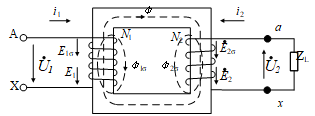
\includegraphics[width=0.80\textwidth]{3-8g.png}
	\caption{变压器负载运行的示意图}
	\label{fig_3.8}
\end{figure}

负载运行时,一次侧磁动势和二次侧磁动势都同时作用在同一磁路上,磁动势${{\dot{F}}_{2}}$的出现使主磁通趋于改变,电动势${{\dot{E}}_{1}}$和${{\dot{E}}_{2}}$也跟着变化,从而打破了原来的平衡状态。在一定的电网电压${{\dot{U}}_{1}}$作用下,${{\dot{E}}_{1}}$的改变使一次侧的电流变化,从空载时的${{\dot{I}}_{0}}$改变为负载时的${{\dot{I}}_{2}}$。这时一、二次侧电流${{\dot{I}}_{1}}$和${{\dot{I}}_{2}}$所产生的磁动势${{\dot{I}}_{1}}{{N}_{1}}$和${{\dot{I}}_{2}}{{N}_{2}}$构成变压器铁心中的合成磁动势${{\dot{F}}_{m}}={{\dot{I}}_{1}}{{N}_{1}}+{{\dot{I}}_{2}}{{N}_{2}}$,而由${{\dot{F}}_{m}}$建立负载时的主磁通$\dot{\Phi }$ (此值与空载时稍有不同),并由$\dot{\Phi }$在一、二次侧感应电动势${{\dot{E}}_{1}}$和${{\dot{E}}_{2}}$。变化的${{\dot{E}}_{1}}$又迫使${{\dot{I}}_{1}}$随之改变,直到变压器中的电磁关系达到新的平衡为止。

一、二次侧电流在各自绕组中还产生漏磁通、感应漏磁电动势。通常把漏磁电动势写成漏抗压降形式,推导方法同上节,即
\begin{equation}
\begin{aligned}
& -{{{\dot{E}}}_{1\sigma }}=\text{j}{{x}_{1\sigma }}{{{\dot{I}}}_{1}} \\ 
& -{{{\dot{E}}}_{2\sigma }}=\text{j}{{x}_{2\sigma }}{{{\dot{I}}}_{2}} \\ 
\end{aligned}
\label{2-16}
\end{equation}

式中 ${{x}_{1\sigma }}$、${{x}_{2\sigma }}$——一、二次侧的漏抗。

一、二次侧还在各自的绕组中产生电阻压降${{\dot{I}}_{1}}{{r}_{1}}$及${{\dot{I}}_{2}}{{r}_{2}}$。

综上所述,变压器负载运行时所发生的电磁关系见图\ref{fig_3.9}。
\begin{figure}[H]
	\centering
	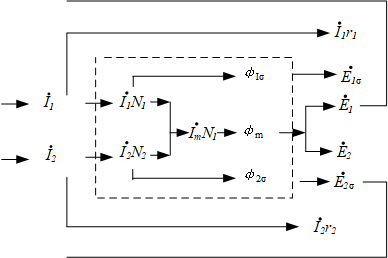
\includegraphics[width=0.80\textwidth]{3-9g.png}
	\caption{变压器负载运行时的电磁关系}
	\label{fig_3.9}
\end{figure}

\subsection{基本方程式}
\subsubsection{电压平衡方程式}
按上述分析,根据图\ref{fig_3.8}所规定的各物理量的正方向,利用电路规律,便可写出变压器负载运行时的一、二次侧的电压平衡方程式,即
\begin{equation}
{{\dot{U}}_{1}}=-\left( {{{\dot{E}}}_{1}}+{{{\dot{E}}}_{1\sigma }} \right)+{{\dot{I}}_{1}}{{r}_{1}}=\left( -{{{\dot{E}}}_{1}} \right)+{{\dot{I}}_{1}}{{r}_{1}}+\text{j}{{\dot{I}}_{1}}{{x}_{1\sigma }}=\left( -{{{\dot{E}}}_{1}} \right)+{{\dot{I}}_{1}}{{Z}_{1}}
\label{2-17}
\end{equation}

\begin{equation}
{{\dot{U}}_{2}}=\left( {{{\dot{E}}}_{2}}+{{{\dot{E}}}_{2\sigma }} \right)-{{\dot{I}}_{2}}{{r}_{2}}={{\dot{E}}_{2}}-{{\dot{I}}_{2}}{{r}_{2}}-\text{j}{{\dot{I}}_{2}}{{x}_{2\sigma }}={{\dot{E}}_{2}}-{{\dot{I}}_{2}}{{Z}_{2}}
\label{2-18}
\end{equation}
或
\begin{equation}
{{\dot{E}}_{2}}={{\dot{U}}_{2}}+{{\dot{I}}_{2}}{{Z}_{2}}
\label{2-19}
\end{equation}

\begin{equation}
{{\dot{U}}_{2}}={{\dot{I}}_{2}}{{Z}_{L}}
\label{2-20}
\end{equation}

上述式中的${{Z}_{1}}={{r}_{1}}+\text{j}{{x}_{1\sigma }}$和${{Z}_{2}}={{r}_{2}}+\text{j}{{x}_{2\sigma }}$分别为一、二次侧的漏阻抗,均为常数,与电流的大小无关。

由于变压器的${{Z}_{1}}$和${{Z}_{2}}$值都比较小,故有${{\dot{U}}_{1}}\approx \left( -{{{\dot{E}}}_{1}} \right)$,${{\dot{U}}_{2}}\approx {{\dot{E}}_{2}}$。因此,变压器负载 后仍近似有式\eqref{2-9}的关系,即
\[\frac{{{U}_{1}}}{{{U}_{2}}}\approx \frac{{{E}_{1}}}{{{E}_{2}}}=k\]

\subsubsection{磁动势平衡方程式}
在图\ref{fig_3.8}中,按全电流定律,可得出变压器负载时一、二次侧磁动势的平衡方程式为
\begin{equation}
{{\dot{F}}_{1}}+{{\dot{F}}_{2}}={{\dot{F}}_{m}}
\label{2-21}
\end{equation}

负载时的主磁通${{\dot{\Phi }}_{m}}$是由合成磁动势${{\dot{F}}_{m}}$建立的。由于${{\dot{\Phi }}_{m}}=\frac{E}{4.44f{{N}_{1}}}\approx \frac{{{U}_{1}}}{4.44f{{N}_{1}}}$基本不变,所以${{\dot{F}}_{m}}$近似等于空载磁动势${{I}_{0}}{{N}_{1}}$。如认为${{\dot{F}}_{m}}$仍由一次侧电流产生,即将一次侧电流${{\dot{I}}_{1}}$看成两个分量,其中一个分量${{\dot{I}}_{m}}$所产生磁动势${{\dot{I}}_{m}}{{N}_{1}}$恰等于合成磁动势${{\dot{F}}_{m}}$,则磁动势平衡方程式可写为
\begin{equation}
{{\dot{I}}_{1}}{{N}_{1}}+{{\dot{I}}_{2}}{{N}_{2}}={{\dot{I}}_{m}}{{N}_{1}}
\label{2-22}
\end{equation}
式中 ${{I}_{m}}$——一次侧电流的励磁分量。

磁动势平衡方程式表明,在负载运行时,一次侧磁动势将随二次侧磁动势的改变而改变,以维持合成磁动势基本不变。

由磁动势平衡方程式可以求得一、二次侧电流间的制约关系。将式(\ref{2-22})除以${{N}_{1}}$并移项得

\begin{equation}
{{\dot{I}}_{1}}={{\dot{I}}_{m}}+\left( -{{{\dot{I}}}_{2}}\frac{{{N}_{2}}}{{{N}_{1}}} \right)={{\dot{I}}_{m}}+{{\dot{I}}_{1\text{L}}}
\label{2-23}
\end{equation}

式中${{\dot{I}}_{1\text{L}}}$——一次侧电流的负载分量,${{\dot{I}}_{1\text{L}}}=-{{\dot{I}}_{2}}\frac{{{N}_{2}}}{{{N}_{1}}}$。

式\eqref{2-23}表明,当有负载电流${{\dot{I}}_{2}}$时,一次侧电流应包含有两个分量。其中励磁分量${{\dot{I}}_{m}}$用以激励主磁通,而负载分量${{\dot{I}}_{1\text{L}}}$所产生磁动势用以抵消二次侧磁动势对主磁路的影响,即
\begin{equation}
{{\dot{I}}_{1\text{L}}}{{N}_{1}}=-{{\dot{I}}_{2}}{{N}_{2}}
\label{2-24}
\end{equation}

式\eqref{2-23}和式\eqref{2-24}是分析变压器一、二次侧电流关系的重要依据。

可见,变压器由空载变到负载运行时,一次侧电流中除保持一个与空载电流${{\dot{I}}_{0}}$接近相等的励磁分量外,还增加一个与二次侧电流成正比的负载分量${{\dot{I}}_{1\text{L}}}$。${{\dot{I}}_{1\text{L}}}$与${{\dot{I}}_{2}}$相位相反,二者的有效值之比为
\begin{equation}
\frac{{{I}_{1\text{L}}}}{{{I}_{2}}}=\frac{{{N}_{2}}}{{{N}_{1}}}=\frac{1}{k}
\label{2-25}
\end{equation}

当${{I}_{m}}$可忽略(${{I}_{m}}\ll {{I}_{1}}$)时,${{I}_{1}}\approx {{I}_{1\text{L}}}$,有

\begin{equation}
\frac{{{I}_{1}}}{{{I}_{2}}}\approx \frac{1}{k}
\label{2-26}
\end{equation}


\subsection{相量图}
假设二次侧的${{\dot{U}}_{2}}$、${{\dot{I}}_{2}}$、$\cos {{\varphi }_{2}}$ 及变比$k$ 为已知,负载时变压器的相量图可按照下述方法控制。

先选用适当的比例尺绘出二次侧电压相量${{\dot{U}}_{2}}$及电流相量${{\dot{I}}_{2}}$,它们之间的夹角就是功率函数角${{\varphi }_{2}}$,根据二次侧电压平衡方程式[见式(\ref{2-19})],得到二次侧的感应电动势${{\dot{E}}_{2}}$。而主磁通相量${{\dot{\Phi }}_{m}}$超前于电动势${{\dot{E}}_{2}}{{90}^{\text{o}}}$。考虑铁损耗之后,励磁电流${{\dot{I}}_{m}}$超前于磁通$\alpha $角度。根据${{\dot{I}}_{1}}={{\dot{I}}_{m}}+{{\dot{I}}_{1\text{L}}}={{\dot{I}}_{m}}+\left( -\frac{{{{\dot{I}}}_{2}}}{k} \right)$可绘出${{\dot{I}}_{1}}$。再根据式(\ref{2-11})求得一次侧感应电动势${{E}_{1}}=k{{E}_{2}}$,可绘出$\left( -{{{\dot{E}}}_{1}} \right)$,最后根据一次侧电压平衡方程${{\dot{U}}_{1}}=\left( -{{{\dot{E}}}_{1}} \right)+{{\dot{I}}_{1}}{{r}_{1}}+\text{j}{{\dot{I}}_{1}}{{x}_{1\sigma }}$,便可绘出一次侧电压${{\dot{U}}_{1}}$。

在图\ref{fig_3.10}所示的变压器向量图中,变压器的变比$k=2$。

\begin{figure}[H]
	\centering
	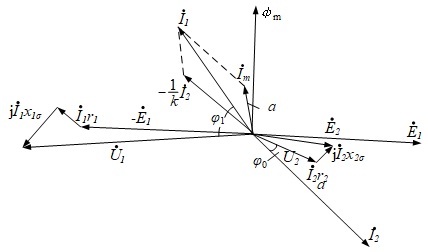
\includegraphics[width=0.80\textwidth]{3-10g.png}
	\caption{变压器相量图}
	\label{fig_3.10}
\end{figure}

\subsection{变压器的能量转换过程}
变压器的能量转换和传递是通过三个平衡完成的。即通过一次侧的电压平衡方程由电源取得电能,再通过磁动势平衡将能量由一次侧传送到二次侧,最后通过二次侧的电压平衡将电能输出到负载。

一次侧的电压平衡决定着输入电流${{\dot{I}}_{1}}$,二次侧的电压平衡决定着输出电流${{\dot{I}}_{2}}$,${{\dot{I}}_{1}}$和${{\dot{I}}_{2}}$通过磁动势平衡影响着主磁通${{\dot{\Phi }}_{m}}$,反过来,${{\dot{\Phi }}_{m}}$所产生的${{\dot{E}}_{1}}$和${{\dot{E}}_{2}}$又通过电压平衡影响着${{\dot{I}}_{1}}$和${{\dot{I}}_{2}}$。可见,这三个平衡不是彼此独立的,而是相互制约的。

变压器运行时,二次侧的电压取决于一次侧电压,即${{U}_{2}}\approx \frac{1}{k}{{U}_{1}}$。输出电流、功率和功率因数取决于二次侧所接的负载,而一次侧的输入电流、功率和功率因数则取决于二次侧的对应量。当变压器满载或接近满载时,${{I}_{1}}\approx \frac{1}{k}{{I}_{2}}$,${{P}_{1}}$略大于${{P}_{2}}$,$\cos {{\varphi }_{1}}$略小于$\cos {{\varphi }_{2}}$ (见图\ref{fig_3.10}。


\section{变压器的等效电路}
通过前面的分析,得出了变压器的各种关系式,将这些基本方程式联立求解就可对变压器进行定量的分析计算。但是这个过程是非常繁琐的,特别是由磁动势到磁通是非线性关系,使得分析计算更加复杂。为了简化分析,人们设想把一、二次侧归纳到一个电路中去,并把磁路对电路的影响也体现在这个电路中。

\subsection{绕组的归算}
为了将变压器的一、二次侧直接连成一个电路,首先要将其华为一个变比$k=1$的假想变压器,为此必须进行绕组的归算。

绕组的归算有两种:一种是保持一次侧匝数${{N}_{1}}$ 不变,设想有一个匝数为${{{N}'}_{2}}={{N}_{1}}$的二次侧,用它来取代原有匝数为${{N}_{2}}$的二次侧;另一种是保持二次侧匝数${{N}_{2}}$不变,设想有一个匝数为${{{N}'}_{1}}={{N}_{2}}$的一次侧,用它来取代原有的匝数为${{N}_{1}}$的一次侧。前一种方法称为二次侧归算到一次侧,后一种方法称为一次侧归算到二次侧。

下面以二次侧归算到一次侧为例,介绍归算的原则和具体办法。二次侧归算后的各种量和参数都将不同于归算前,但对其磁路和一次侧电路的作用不能改变。变压器二次侧对磁路及一次侧电路的影响是通过磁动势${{\dot{F}}_{2}}$体现的,因此保持${{\dot{F}}_{2}}$不变是绕组归算的原则。

\subsubsection{二次侧电流的归算值}
根据归算前后的磁动势应保持不变的原则,可求得二次侧电流的归算值为
${{{\dot{I}}'}_{2}}{{{N}'}_{2}}={{\dot{I}}_{2}}{{N}_{2}}$
即
\begin{equation}
{{{\dot{I}}'}_{2}}=\frac{{{N}_{2}}}{{{{{N}'}}_{2}}}{{\dot{I}}_{2}}=\frac{1}{k}{{\dot{I}}_{2}}
\label{2-27}
\end{equation}

\subsubsection{二次侧电动势的归算值}
由于归算前、后主磁场和漏磁场都没有改变,根据电动势和匝数成正比的关系,可得
\begin{equation}
\left. \begin{aligned}
& \frac{{{{{\dot{E}}'}}_{2}}}{{{{\dot{E}}}_{2}}}=\frac{{{N}_{1}}}{{{N}_{2}}}=k \\ 
& {{{{\dot{E}}'}}_{2}}=k{{{\dot{E}}}_{2}}={{{\dot{E}}}_{1}} \\ 
\end{aligned} \right\}
\label{2-28}
\end{equation}

\begin{equation}
\left. \begin{aligned}
& \frac{{{{{\dot{E}}'}}_{2\sigma }}}{{{{\dot{E}}}_{2\sigma }}}=\frac{{{N}_{1}}}{{{N}_{2}}}=k \\ 
& {{{{\dot{E}}'}}_{2\sigma }}=k{{{\dot{E}}}_{2\sigma }} \\ 
\end{aligned} \right\}
\label{2-29}
\end{equation}

\subsubsection{二次侧漏抗的归算值}
根据漏电抗定义,可得
\begin{equation}
{{{x}'}_{2}}=\frac{-{{{{\dot{E}}'}}_{2\sigma }}}{j{{{{\dot{I}}'}}_{2}}}=\frac{-k{{{\dot{E}}}_{2\sigma }}}{j\frac{1}{k}{{{\dot{I}}}_{2}}}={{k}^{2}}\left( -\frac{{{{\dot{E}}}_{2\sigma }}}{j{{{\dot{I}}}_{2}}} \right)={{k}^{2}}{{x}_{2\sigma }}
\label{2-30}
\end{equation}

\subsubsection{二次侧电阻的归算值}
由于归算后绕组的匝数从${{N}_{2}}$变为${{N}_{1}}$,线圈总长度应变为原来的$\frac{{{N}_{1}}}{{{N}_{2}}}$倍,又由于归算后的电流由${{I}_{2}}$变为${{{I}'}_{2}}=\frac{1}{k}{{I}_{2}}$,导线的截面积应变为原来的$\frac{{{N}_{2}}}{{{N}_{1}}}$倍。这样,根据导线电阻与其长度成正比,而与其截面积成反比,可得
\begin{equation}
{{{r}'}_{2}}={{\left( \frac{{{N}_{1}}}{{{N}_{2}}} \right)}^{2}}{{r}_{2}}={{k}^{2}}{{r}_{2}}
\label{2-31}
\end{equation}
随之可得
\begin{equation}
{{{Z}'}_{2}}={{{r}'}_{2}}+j{{{x}'}_{2\sigma }}={{k}^{2}}\left( {{r}_{2}}+j{{x}_{2\sigma }} \right)={{k}^{2}}{{Z}_{2}}
\label{2-32}
\end{equation}

\subsubsection{二次侧电压的归算值}
根据归算后二次侧的电压方程式可得
\begin{equation}
{{{\dot{U}}'}_{2}}={{{\dot{E}}'}_{2}}-{{{\dot{I}}'}_{2}}{{{Z}'}_{2}}=k{{\dot{E}}_{2}}-\frac{1}{k}{{\dot{I}}_{2}}{{k}^{2}}{{Z}_{2}}=k\left( {{{\dot{E}}}_{2}}-{{{\dot{I}}}_{2}}{{Z}_{2}} \right)=k{{\dot{U}}_{2}}
\label{2-33}
\end{equation}

\subsubsection{负载阻抗的归算值}
从阻抗为电压与电流之比可得
\begin{equation}
{{{Z}'}_{L}}=\frac{{{{{\dot{U}}'}}_{2}}}{{{{{\dot{I}}'}}_{2}}}=\frac{k{{{\dot{U}}}_{2}}}{\frac{1}{k}{{{\dot{I}}}_{2}}}={{k}^{2}}\frac{{{{\dot{U}}}_{2}}}{{{{\dot{I}}}_{2}}}={{k}^{2}}{{Z}_{L}}
\label{2-34}
\end{equation}
综上所述,当把二次侧各物理量归算到一次侧时,电动势、电压的归算值等于其原来的数值乘以 $k$;电阻、电抗、阻抗的归算值等于其原来的数值乘以${{k}^{2}}$;电流的归算值则等于原来的数值乘以$\frac{1}{k}$。

从能量关系看,归算后二次侧的铜损耗为$\dot I_2^{\prime2}{r'_2} = {\frac{1} {{k^2}}}I_2^2{k^2}{r_2} = I_2^2{r_2}$;输出的视在功率为(公式有地方不清楚,请确认):${{{U}'}_{2}}=k{{U}_{2}}\frac{1}{k}{{I}_{2}}={{U}_{2}}{{I}_{2}}$。可见,归算后的功率和损耗仍和归算前一样,没有改变。

\subsection{励磁阻抗}
在变压器运行时,从电磁感应关系看,励磁电流${{I}_{m}}$建立主磁通${{\dot{\Phi }}_{m}}$,交变的主磁通${{\dot{\Phi }}_{m}}$在一次侧产生感应电动势,并在铁心中产生一定的铁损耗。如能把主磁通对电路的上述影响设法直接体现在电路中,则可得到变压器运行时的等效电路,使分析得到简化。

在前面把漏磁通在电路中的作用看做是电流流过漏感抗所形成的电压降[见式\eqref{2-16}]。同样,对于主磁通${{\dot{\Phi }}_{m}}$在电路中的作用,也可类似地引入一个参数来表达。考虑到主磁通在 铁心中引起铁损耗,因此不能只引入一个电抗,而是应引入一个包含一定电阻的阻抗${{Z}_{m}}$,它与产生${{\dot{\Phi }}_{m}}$的${{\dot{I}}_{m}}$和${{\dot{\Phi }}_{m}}$所产生的感应电动势${{\dot{E}}_{1}}$之间的关系为
\begin{equation}
-{{\dot{E}}_{1}}={{\dot{I}}_{m}}{{Z}_{m}}
\label{2-35}
\end{equation}
$$
{{Z}_{m}}={{r}_{m}}+j{{x}_{m}}
$$
式中${{Z}_{m}}$——变压器的励磁阻抗;

${{x}_{m}}$——励磁电抗;

${{r}_{m}}$——励磁电阻,它是对应于铁损耗的等效电阻,即$I_{m}^{2}{{r}_{m}}={{p}_{Fe}}$。

由于磁化曲线呈非线性,参数${{Z}_{m}}$随电压变化,它不是常数。但变压器正常运行时,外延电压总是等于或接近等于额定电压,在这种情况下,也可把${{Z}_{m}}$看成常数。

\subsection{等效电路}
归算后变压器的基本方程式为
\begin{equation}
\left. \begin{aligned}
& {{{\dot{U}}}_{1}}\text{=}-{{{\dot{E}}}_{1}}\text{+}{{{\dot{I}}}_{1}}{{Z}_{1}} \\ 
& {{{{\dot{U}}'}}_{2}}\text{=}{{{{\dot{E}}'}}_{2}}-{{{{\dot{I}}'}}_{2}}{{{{Z}'}}_{2}} \\ 
& {{{\dot{I}}}_{m}}\text{=}{{{\dot{I}}}_{1}}\text{+}{{{{\dot{I}}'}}_{2}} \\ 
& {{{\dot{E}}}_{1}}={{{{\dot{E}}'}}_{2}} \\ 
& -{{{\dot{E}}}_{1}}\text{=}{{{\dot{I}}}_{m}}{{Z}_{m}} \\ 
& {{{{\dot{U}}'}}_{2}}\text{=}{{{{\dot{I}}'}}_{2}}{{{{Z}'}}_{L}} \\ 
\end{aligned} \right\}
\label{2-36}
\end{equation}

按上式给出的各种关系,就可绘出一个准确代表真实变压器的等效电路。

\subsubsection{T形等效电路}
变压器等效电路的演变过程如图(\ref{fig_3-11})所示。在图\ref{fig_3-11}(a)中,一次侧回路串联电阻${{r}_{1}}$及电抗${{x}_{1\sigma }}$来代表一次侧内部的电阻和漏抗;同样,二次侧回路串联电阻${{r}_{2}}$及电抗${{x}_{2\sigma }}$来代表二次侧内部的电阻及漏抗。这样,一、二次侧就可以看成是没有电阻和漏抗的两个理想绕组,绕组中只有由主磁通感生的电动势${{\dot{E}}_{1}}$及${{\dot{E}}_{2}}$。经过归算之后,${{\dot{E}}_{1}}={{{\dot{E}}'}_{2}}$,于是得到图(\ref{fig_3-11}(b))。既然一、二次侧的感应电动势相等,故可以把它们之间的等电位点连接起来,而不会改变变压器内部的电磁关系。这样两个绕组便可合二为一而得到图(\ref{fig_3-11}(c))。显然这个绕组中流过的电流便是${{\dot{I}}_{m}}={{\dot{I}}_{1}}+{{{\dot{I}}'}_{2}}$,它产生感应电动势$(-{{{\dot{E}}'}_{2}})=(-{{\dot{E}}_{1}})={{\dot{I}}_{m}}{{Z}_{m}}$。将这个绕组用励磁阻抗${{Z}_{m}}={{r}_{m}}+j{{x}_{m}}$来代替,于是便得到图\ref{fig_3.12}所示等效电路图,称为 T 形等效电路图。

应当指出,利用等效电路图所求得的二次侧电压、电流均为归算到一次侧的值,如要得到其实际值,还需进行反归算。
\begin{figure}[H]
	\centering
	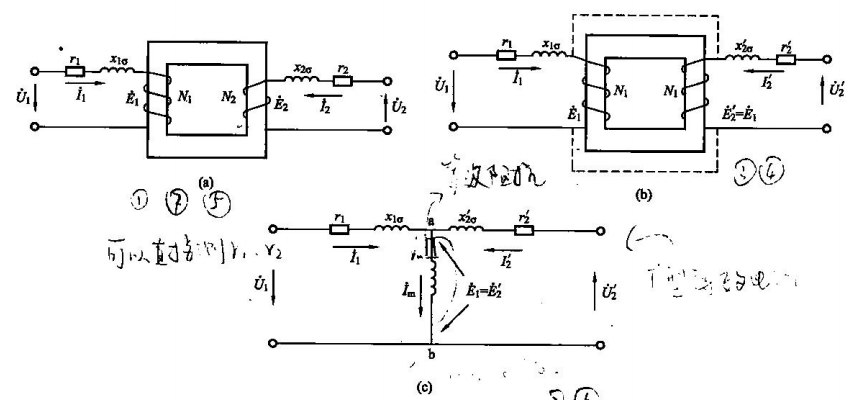
\includegraphics[width=0.80\textwidth]{3-11.png}
	\caption{变压器的等效电路的演变过程
		(a)绕组中只有${{\dot{E}}_{1}}$及${{\dot{E}}_{2}}$;(b)${{\dot{E}}_{1}}={{{\dot{E}}'}_{2}}$;(c)等效电路}
	\label{fig_3-11}
\end{figure}
\begin{figure}[H]
	\centering
	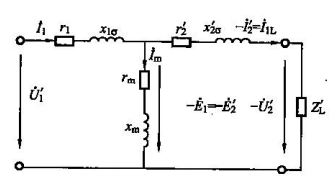
\includegraphics[width=0.80\textwidth]{3-12.png}
	\caption{T形等效电路}
	\label{fig_3.12}
\end{figure}

\subsubsection{近似等效电路}
T形等效电路能准确地代表实际的变压器,但它含有串联和并联支路,进行复数运算仍比较复杂。如将T形等效电路中的励磁支路从中间移到电源端(见图\ref{fig:3.13}),则电路中只有并联关系,可使分析汁算大为简化。

这样改动后,${{\dot{I}}_{m}}$少经过一个阻抗${{{Z}}_{1}}$,会变大;${{{Z}}_{1}}$上少了一部分压降${{\dot{I}}_{m}}{{Z}_{1}}$,后面电压会有所升高。但由于${{\dot{I}}_{m}}\ll {{\dot{I}}_{1N}}$,$\left| {{Z}_{1}} \right|\ll \left| {{Z}_{m}} \right|$,所以${{{I}}_{m}}$和${{{I}'}_{2}}$的值增大都非常微小。改动后的电路称为近似等效电路。
\begin{figure}  %两个图片并排放
	\begin{minipage}[H]{0.45\linewidth}  
		\centering  
		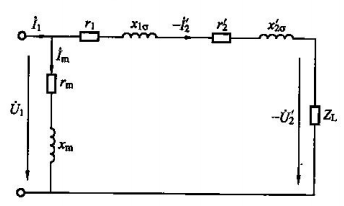
\includegraphics[width=2.2in]{3-13.png}  
		\caption{变压器的近似等效电路}
		\label{fig:3.13} 
	\end{minipage}
	\begin{minipage}[H]{0.45\linewidth}  
		\centering  
		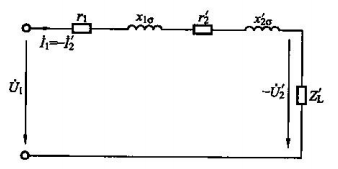
\includegraphics[width=2.2in]{3-14.png}  
		\caption{变压器的简化等效电路} 
		\label{fig:3.14} 
	\end{minipage}
\end{figure}
\subsubsection{简化等效电路}
在电力变压器中,由于 在 中所占的比例很小,在工程中有时可以忽略 ,即在等效电路中去掉励磁支路,而得到一个更简单的无分支电路,如图\ref{fig:3.14}所示,称为变压器的简化等效电路。

在近似等效电路和简化等效电路中,可将一、二次侧的漏阻抗合起来,得到
\begin{equation}
\begin{aligned}
& {{r}_{k}}={{r}_{1}}+{{{{r}'}}_{2}} \\ 
& {{x}_{k}}={{x}_{1\sigma }}+{{{{x}'}}_{2\sigma }} \\ 
& {{Z}_{k}}={{r}_{k}}+j{{x}_{k}}={{Z}_{1}}+{{{{Z}'}}_{2}} 
\end{aligned}
\label{2-37}
\end{equation}

式中  ${{Z}_{k}}$——变压器的短路阻抗;

${{r}_{k}}$——短路电阻;

${{x}_{k}}$——短路电抗。

基本方程式、等效电路和相量图是分析变压器的三种工具,在进行定量分析时需要使用等效电路;讨论各物理量之间的大小和相位关系时,相量图比较方便。

\subsection{变压器参数的测定}
为了对变压器进行定量的分析计算,必须先知道变压器的各种参数,变压器的参数可以 通过空载试验和短路试验求取。

\subsection{空载试验}
通过空载试验可测定变压器的励磁参数,同时还可测定变压器的变比和铁损耗。由于励 磁阻抗的大小与磁路的饱和程度有关,铁损耗也与主磁通大小相关,所以空载试验应在额定 电压下进行。为了安全和便于测量,通常将变压器的低压侧接电源,高压侧开路,接线图如图\ref{fig_3.15}所示。

根据仪表读数可测量电压${{U}_{1N}}$和${{U}_{20}}$、空载电流${{I}_{0}}$及空载损耗${{p}_{0}}$。对于三相变压器,测得的电压、电流皆为线值,损耗为三相值,在用其求励磁参数时必须先将它们化为每相值。

图\ref{fig_3.16}所示为变压器空载时的等效电路,由于${{x}_{m}}\gg {{x}_{1\sigma }}$,${{r}_{m}}\gg {{r}_{1}}$,所以空载总阻抗${{Z}_{0}}={{Z}_{m}}+{{Z}_{1}}\approx {{Z}_{m}}$,${{p}_{0}}=I_{0}^{2}{{r}_{m}}+I_{0}^{2}{{r}_{1}}\approx I_{0}^{2}{{r}_{m}}$。
\begin{figure}[H]
	\centering
	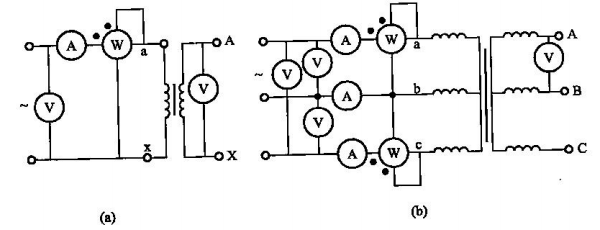
\includegraphics[width=0.80\textwidth]{3-15.png}
	\caption{变压器空载试验接线图}
	\label{fig_3.15}
\end{figure}
\begin{figure}[H]
	\centering
	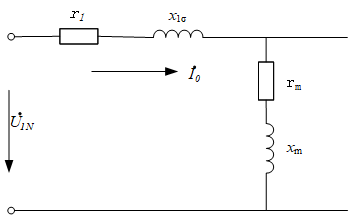
\includegraphics[width=0.80\textwidth]{3-16g.png}
	\caption{变压器空载时的等效电路}
	\label{fig_3.16}
\end{figure}
变压器励磁参数的计算式为
\begin{equation}
\begin{aligned}
& \left| {{Z}_{m}} \right|\approx \left| {{Z}_{0}} \right|=\frac{{{U}_{1N}}}{{{I}_{0}}} \\ 
& {{r}_{m}}\approx {{r}_{0}}=\frac{{{p}_{0}}}{I_{0}^{2}} \\ 
& {{x}_{m}}=\sqrt{{{\left| {{Z}_{m}} \right|}^{2}}-r_{m}^{2}} 
\end{aligned}
\label{2-38}
\end{equation}

式(\ref{2-38})给出的都是对变压器低压侧的数值,如要得到变压器高压侧的励磁参数,则应将以上数据分别乘以变比$k$的平方。在忽略一次侧微小的铜损耗$I_{0}^{2}{{r}_{1}}$的条件下,变压器在额定电压下的铁损耗近似等于空载损耗,即
\begin{equation}
{{p}_{Fe}}=I_{0}^{2}{{r}_{m}}\approx {{p}_{0}}
\label{2-39}
\end{equation}
变压器的变比为
\begin{equation}
k=\frac{{{U}_{20}}(high voltage)}{{{U}_{1N}}( low voltage)}
\label{2-40}
\end{equation}

\subsubsection{短路试验}
通过短路试验可测定变压器的短路参数和铜损耗,为避免短路电流过大,外施电压${{U}_{k}}$应远小于一次侧的额定电压${{U}_{1N}}$。一般取使${{I}_{k}}={{I}_{1N}}$时的${{U}_{k}}$进行试验,这时的${{U}_{k}}$大约是额定电压${{U}_{1N}}$的5\%\textasciitilde10\%。为便于测量,通常将额定电流较小的高压侧接电源,低压侧直接短路,接线图如图\ref{fig_3.17}所示。

根据仪表读数可测得短路电压${{U}_{k}}$、短路电流${{I}_{k}}$及短路损耗${{p}_{k}}$。由于\[{{U}_{k}}\ll {{U}_{1N}}\],铁心中磁通很小,励磁电流可以略去,故短路试验时的等效电路为图\ref{fig_3.18}所示的简化等效电路。

变压器短路参数的计算式为
\begin{equation}
\begin{aligned}
& \left| {{Z}_{k}} \right|=\frac{{{U}_{k}}}{{{I}_{k}}} \\ 
& {{r}_{k}}=\frac{{{p}_{k}}}{I_{k}^{2}} \\ 
& {{x}_{k}}=\sqrt{{{\left| {{Z}_{k}} \right|}^{2}}-r_{k}^{2}} 
\end{aligned}
\label{2-41}
\end{equation}

对于三相变压器,应先将测量值都化为每相值,然后再用式(\ref{2-41})计算。由于绕组的电阻随温度而变化,而短路试验一般是在室温下进行,故应将测得的电阻换算到标准工作 温度时的数值。按国家标准,油浸式电力变压器的短路阻抗应换算到75℃的数值。

短路试验时的输入功率${{p}_{k}}$,包括一、二次侧的铜损耗和铁心中的铁损耗。由于铁心中磁通很小,铁损耗可以略去,故可认为短路损耗${{p}_{k}}$全都是一、二次侧的额定铜损耗${{p}_{\text{Cu}N}}$,即
\begin{equation}
{{p}_{\text{Cu}N}}=I_{1N}^{2}{{r}_{1}}+I_{2N}^{2}{{r}_{2}}=I_{1N}^{2}{{r}_{1}}+{I}\prime_{2N}^{2}{{{r}'}_{2}}=I_{k}^{2}{{r}_{k}}={{p}_{k}}
\label{2-42}
\end{equation}

\subsubsection{短路电压}
在短路试验中,使短路电流${{I}_{k}}={{I}_{1N}}$,这时的外施电压${{U}_{k}}$与额定电压${{U}_{1N}}$的比值的百分数,定义为变压器的短路电压${{u}_{k}}$,即
\begin{equation}
{{u}_{k}}=\frac{{{U}_{k}}}{{{U}_{1N}}}\times 100\%
\label{2-43}
\end{equation}
\begin{figure}[H]
	\centering
	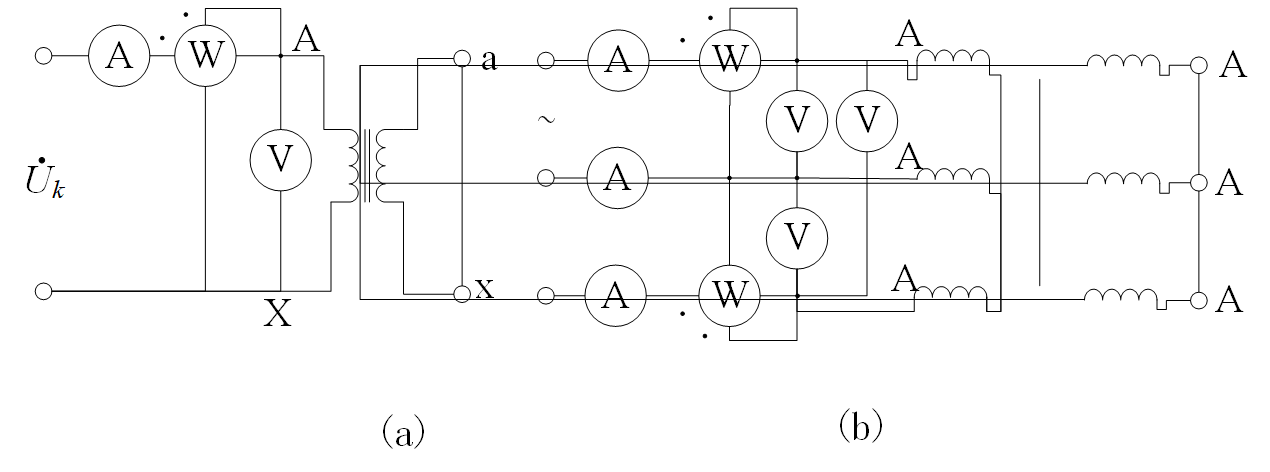
\includegraphics[width=0.80\textwidth]{3-17g.png}
	\caption{变压器短路试验接线图
		(a)单相;(b)三相}
	\label{fig_3.17}
\end{figure}
\begin{figure}[H]
	\centering
	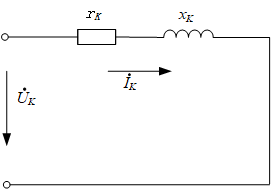
\includegraphics[width=0.80\textwidth]{3-18g.png}
	\caption{短路试验的等效电路}
	\label{fig_3.18}
\end{figure}
由等效电(见图\ref{fig_3.18})可知,${{U}_{k}}={{I}_{k}}\left| {{Z}_{k}} \right|={{I}_{1N}}\left| {{Z}_{k}} \right|$,代人式\eqref{2-43}得
\begin{equation}
{{u}_{k}}=\frac{\left| {{Z}_{k}} \right|{{I}_{1N}}}{{{U}_{1N}}}={{\left| {{Z}_{k}} \right|}^{*}}\times 100\%
\label{2-44}
\end{equation}
它的有功分量和无功分量分别为
\begin{equation}
\begin{aligned}
& {{u}_{kr}}=\frac{{{r}_{k}}{{I}_{1N}}}{{{U}_{1N}}}=r_{k}^{*}\times 100% \\ 
& {{u}_{kx}}=\frac{{{x}_{k}}{{I}_{1N}}}{{{U}_{1N}}}=x_{k}^{*}\times 100% \\ 
\end{aligned} 
\label{2-45}
\end{equation}

可见,变压器的短路电压${{u}_{k}}$等于其短路阻抗的标幺值(见下节),它反映着变压器短路 阻抗的大小,故又称阻抗电压。${{u}_{k}}$是标在变压器铭牌上的一个重要数据。${{u}_{k}}$越小,变压器运行时输出电压的波动越小,但发生短路时的短路电流越大。

\subsection{标幺值}
在工程计算中,各种物理量如电压、电流、阻抗、功率等,有时不使用它们的实际值,而把这些物理量表示成与某一选定的基值之比的形式,称为标幺值。在电机中,常取各种物理量的额定值作为基值。标幺值的表示方法是,原物理量符号的右上角加“*”。

(1)一次侧电压基值为${{U}_{1N}}$,故${{U}_{1}}$的标幺值为$U_{1}^{*}=\frac{{{U}_{1}}}{{{U}_{1N}}}$;

(2)二次侧电压基值为${{U}_{2N}}$,故${{U}_{2}}$的标幺值为$U_{2}^{*}=\frac{{{U}_{2}}}{{{U}_{2N}}}$;

(3)一次侧电流基值为${{I}_{1N}}$,故${{I}_{1}}$的标幺值为$I_{1}^{*}=\frac{{{I}_{1}}}{{{I}_{1N}}}$;

(4)二次侧电流基值为${{I}_{2N}}$,故${{I}_{2}}$的标幺值为$I_{2}^{*}=\frac{{{I}_{2}}}{{{I}_{2N}}}$;

(5)一次侧阻抗基值为${{Z}_{1N}}=\frac{{{U}_{1N}}}{{{I}_{1N}}}$,故${{Z}_{1}}$的标幺值为$Z_{1}^{*}=\frac{{{Z}_{1}}}{{{Z}_{1N}}}=\frac{{{Z}_{1}}{{I}_{1N}}}{{{U}_{1N}}}$

(6)二次侧阻抗基值为${{Z}_{2N}}=\frac{{{U}_{2N}}}{{{I}_{2N}}}$,故${{Z}_{2}}$的标幺值为$Z_{2}^{*}=\frac{{{Z}_{2}}}{{{Z}_{2N}}}=\frac{{{Z}_{2}}{{I}_{2N}}}{{{U}_{2N}}}$

采用标幺值具有下列优点: 

(1)对于不同容量的变压器,其实际值可能相差甚大,但如用标幺值表示时则较为接近。因此采用标幺值时它们的参数及性能数据便于进行比较,同时可以根据标幺值的大小来判断变压器性能的优劣。

(2)采用标幺值时,各物理量在归算前、后的数值相等。例如
$$r_{2}^{*}=\frac{{{I}_{2N}}}{{{U}_{2N}}}{{r}_{2}}=\frac{{{I}_{2N}}{{U}_{2N}}{{r}_{2}}}{U_{2N}^{2}}=\frac{{{U}_{1N}}{{I}_{1N}}{{r}_{2}}}{U_{1N}^{2}/{{k}^{2}}}=\frac{{{I}_{1N}}{{k}^{2}}{{r}_{2}}}{U_{1N}^{{}}}=\frac{{{I}_{1N}}{{{{r}'}}_{2}}}{U_{1N}^{{}}}={r}\prime_{2}^{*}$$
这里要注意,二次侧归算到一次侧后的物理量的基值取一次侧的额定值。因此,采用标幺值时不需要进行归算。

(3)采用标幺值后,可避免冗繁的数字计算,从而可以减小运算误差。

\subsection{变压器的主要运行特性}
\subsection{变压器的电压变化率}
当变压器空载运行时,一次侧加额定电压${{U}_{1N}}$,二次侧电压${{U}_{20}}$基本上等于其额定电压${{U}_{2N}}$。负载后,由于变压器一、二次侧的漏阻抗压降,致使二次侧电压${{U}_{2}}$与空载电压${{U}_{20}}$不相等。从空载到满载二次侧电压的算术差${{U}_{20}}-{{U}_{2}}$与其额定电压${{U}_{2N}}$的比值定义为变压器的电压变化率,即
\begin{equation}
\Delta U=\frac{{{U}_{20}}-{{U}_{2}}}{{{U}_{2N}}}\times 100\%
\label{2-46}
\end{equation}
将式(\ref{2-46})中的${{U}_{20}}$用${{U}_{2N}}$代替,分子、分母都乘以变比k,则得
\begin{equation}
\Delta U=\frac{{{U}_{1N}}-{{{{U}'}}_{2}}}{{{U}_{1N}}}\times 100\%
\label{2-47}
\end{equation}
\begin{figure}[H]
	\centering
	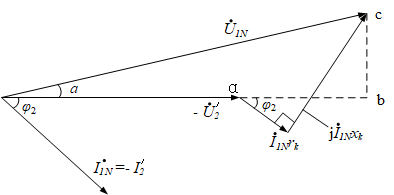
\includegraphics[width=0.80\textwidth]{3-19g.png}
	\caption{由相量图求$\Delta U$}
	\label{fig_3.19}
\end{figure}
应用简化等效电路,则输出电流$(-{{{\dot{I}}'}_{2}})={{\dot{I}}_{1N}}$,输出电压 $(-{{\dot{{U}'}}_{2}})={{\dot{U}}_{1N}}-{{\dot{I}}_{1N}}{{Z}_{k}}$,$-{{\dot{{U}'}}_{2}}$与${{\dot{{U}}}_{1N}}$之间关系如图\ref{fig_3.19}所示。

由图可得${{U}_{1N}}=\sqrt{\left( {{{{\dot{U}}'}}_{2}}+\overline{ab} \right){{}^{2}}+{{\overline{bc}}^{2}}}$实际中${{I}_{1N}}{{r}_{k}}$和 ${{I}_{1N}}{{x}_{k}}$都远小于${{{U}'}_{2}}$,所以${{\dot{U}}_{1N}}$和$-{{\dot{{U}'}}_{2}}$的夹角$\alpha $非常小,它所对线段bc也很小,可以略去。所以
\begin{equation}
{{U}_{1N}}={{{U}'}_{2}}+\overline{ab}
\label{2-48}
\end{equation}
将式(\ref{2-44})带入式(\ref{2-43})得
\begin{equation}
\Delta U=\frac{\overline{ab}}{{{U}_{1N}}}\times 100\%
\label{2-49}
\end{equation}
由图\ref{fig_3.19}所示的几何关系,得
\begin{equation}
\overline{ab}={{I}_{1N}}{{r}_{k}}\cos {{\varphi }_{2}}+{{I}_{1N}}{{x}_{k}}\sin {{\varphi }_{2}}
\label{2-50}
\end{equation}
将式(\ref{2-48})带入式(\ref{2-47})得
\begin{equation}
\begin{aligned}
& \Delta U=\frac{{{I}_{1N}}{{r}_{k}}\cos {{\varphi }_{2}}+{{I}_{1N}}{{x}_{k}}\sin {{\varphi }_{2}}}{{{U}_{1N}}}\times 100% \\ 
& =r_{k}^{*}\cos {{\varphi }_{2}}+x_{k}^{*}\sin {{\varphi }_{2}} \\ 
& =u_{kr}^{{}}\cos {{\varphi }_{2}}+u_{kx}^{{}}\sin {{\varphi }_{2}} \\ 
\end{aligned}
\label{2-51}
\end{equation}

从式(\ref{2-51})可知,$\Delta U$的大小与负载的功率因数有关。当负载为电阻性或感性时, ${{\varphi }_{2}}>0$,此时$\Delta U>0$ ,即随着负载电流的增加二次侧电压下降;当负载为容性时,则${{\varphi }_{2}}<0$,$\sin {{\varphi }_{2}}<0$,如果$\left| {{\varphi }_{2}} \right|$较大,使得$\left| {{u}_{kx}}\sin {{\varphi }_{2}} \right|>\left| {{u}_{kx}}\cos {{\varphi }_{2}} \right|$,则$\Delta U<0$,即二次侧电压随着负载电流的增加而上升。

常用的电力变压器,当${{I}_{2}}={{I}_{2N}}$,$\cos {{\varphi }_{2}}=0.8$(滞后)时,$\Delta U$大约为5\%\textasciitilde8\%。

\subsection{效率}
从等效电路可以看出变压器的功率分配关系和平衡关系。变压器输入功率为
$${{P}_{1}}\text{=}{{U}_{1}}{{I}_{1}}\cos {{\varphi }_{1}}$$

输入功率中的一小部分供给铁心损耗,其值为
\[{{p}_{\text{Fe}}}=I_{\text{m}}^{2}{{r}_{\text{m}}}\]

试验结果说明,在频率不变时铁损耗近似与磁通密度平方成正比,也即与主磁通${{\Phi }_{m}}$ 的平方成正比。如前所述,当负载变化时,铁心中主磁通${{\Phi }_{m}}$的大小变化十分轻微,可以近似认为是常数,因此铁心损耗基本上为一定值,称为不变损耗,可以通过在额定电压下的空载试验求得(即${{p}_{\text{Fe}}}={{p}_{0}}$)。
\begin{figure}[H]
	\centering
	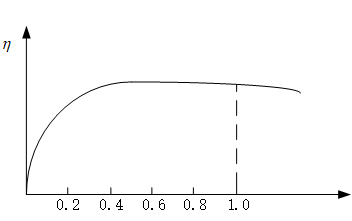
\includegraphics[width=0.80\textwidth]{3-20g.png}
	\caption{变压器的效率曲线}
	\label{fig_3.20}
\end{figure}
输入功率中的另一部分供给一、二次侧的铜损耗,其值为
\begin{equation}
{{p}_{\text{Cu}}}=I_{1}^{2}{{r}_{1}}+I_{2}^{2}{{r}_{2}}
\label{2-52}
\end{equation}

由于铜损耗正比于电流的平方,故称它为可变损耗。如果令$\beta =\frac{{{I}_{2}}}{{{I}_{2N}}}\approx \frac{{{I}_{1}}}{{{I}_{1N}}}$ 表示负载系数${{I}_{1}}=\beta {{I}_{1N}}$ ,${{I}_{2}}=\beta {{I}_{2N}}$。将此关系带入式(\ref{2-52}),得
\begin{equation}
{{p}_{\text{Cu}}}={{\beta }^{2}}I_{1N}^{2}{{r}_{1}}+{{\beta }^{2}}I_{2N}^{2}{{r}_{2}}={{\beta }^{2}}{{p}_{\text{CuN}}}
\label{2-53}
\end{equation}

式中  ${{p}_{\text{CuN}}}$ ——一、二次侧在额定电流时的铜损耗,它可以通过短路试验求得,即(该公式再进行确认一下)${{p}_{\text{CuN}}}={{p}_{\text{kN}}}=I_{1N}^{2}{{r}_{1}}+I_{2N}^{2}{{r}_{2}}$ 

输出功率为
\[{{P}_{2}}={{U}_{2}}{{I}_{2}}\cos {{\varphi }_{2}}\]

通常情况下,负载时变压器二次侧电压${{U}_{2}}$变动很小,可以近似地认为${{U}_{2}}={{U}_{2N}}$,再考虑${{I}_{2}}=\beta {{I}_{2N}}$,于是有
\begin{equation}
{{P}_{2}}=\beta {{U}_{2N}}{{I}_{2N}}\cos {{\varphi }_{2}}=\beta {{S}_{N}}\cos {{\varphi }_{2}}
\label{3-54}
\end{equation}

输入功率应该等于损耗与输出功率之和,所以变压器中的功率平衡方程为
$${{P}_{1}}={{P}_{2}}+{{p}_{\text{Fe}}}+{{p}_{\text{Cu}}}={{P}_{2}}+\sum{p}$$

式中,$\sum{p}$ 称为变压器总损耗。

变压器的效率就是输出功率与输入功率的比值,即
\begin{equation}
\eta =\frac{{{P}_{2}}}{{{P}_{1}}}=\frac{{{P}_{2}}}{{{P}_{2}}+\sum{p}}=\frac{\beta {{S}_{N}}\cos {{\varphi }_{2}}}{\beta {{S}_{N}}\cos {{\varphi }_{2}}+{{p}_{0}}+{{\beta }_{2}}{{p}_{kN}}}
\label{2-55}
\end{equation}

由式(\ref{2-55})可见,当功率因数不变时,变压器的效率将随负载而变化(见图\ref{fig_3.20})。

把式(\ref{2-55})对$\eta $ 微分并使其等于零,可以得到变压器效率最高的条件为
\begin{equation}
{{p}_{0}}={{\beta }^{2}}{{p}_{kN}}
\label{2-57}
\end{equation}

在不损耗与可变损耗相等时,变压器的效率具有最大值。
由于电力变压器的负载时刻变化,但一次侧长期接在电网上,铁损耗总是存在。为了使变压器的平均效率较高,应让变压器的铁损耗小于它的额定铜损耗。一般电力变压器的最大效率发生在$\beta =0.5\tilde{\ }0.6$ 范围内,这时铁损耗与额定铜损耗之比约为$\frac{{{p}_{0}}}{{{p}_{kN}}}=\frac{1}{4}\tilde{\ }\frac{1}{3}$。
\section{小结}
(1)变压器运行时既有主磁通又有漏磁通。建立主磁通是变压器进行能量转换、传递的先决条件。而漏磁通虽不是变压器工作需要,但却是无法避免的,其值远小于主磁通且与产生它的电流成正比,通常用漏抗压降来代表它在绕组中感生电动势的作用。

(2)变压器负载运行时,为维持主磁通${{\Phi }_{m}}$基本不变,一次侧电流${{\dot{I}}_{1}}$将自动随着二次侧电流${{\dot{I}}_{2}}$的变化而变化。可以认为${{\dot{I}}_{1}}$由空载时只有励磁分量${{\dot{I}}_{\text{m}}}\text{=}{{\dot{I}}_{0}}$,变为既有励磁分量${{\dot{I}}_{\text{m}}}$又有与${{\dot{I}}_{2}}$成正比的负载分量${{\dot{I}}_{\text{1L}}}=-\frac{1}{k}{{\dot{I}}_{2}}$。

(3)变压器是通过一次侧的电压平衡、磁动势平衡和二次侧的电压平衡来完成能量转换过程的。这三个平衡之间相互影响,相互制约。

(4)基本方程式、相量图和等效电路是分析变压器的三种工具。前两种主要用于定性分析,而在对变压器进行定量计算时则要使用等效电路。

为了得到等效电路,必须对变压器进行绕组归算,并引入励磁阻抗${{Z}_{m}}$来代表主磁通对电路的影响作用。

(5)通过空载试验,可测定变压器的励磁参数、变比及额定电压下的铁损耗;通过短路实验,可测定变压器的短路参数及额定铜损耗。

(6)使用标幺值,可使变压器的分析、计算得到简化

(7)电压变化率和效率是变压器的两个重要性能指标。电压变化率越小,变压器的供电质量越高;效率越高,变压器运行的经济性越好。

\end{document}